\documentclass[11pt]{article}
\usepackage[utf8]{inputenc}
\usepackage{amsmath}
\usepackage{titlesec}
\usepackage{titling}
\usepackage{geometry}
\usepackage{graphicx}
\usepackage{hyperref}
\usepackage{float}
\usepackage{fancyhdr}
\usepackage{wallpaper}
\usepackage{afterpage} 
\usepackage{pagecolor} 
\usepackage{multirow}
\usepackage{wrapfig}
\usepackage{lipsum} 
\usepackage{url}
\usepackage[toc,page]{appendix}
\usepackage{algorithm}
\usepackage{algpseudocode}
\usepackage{pgfgantt}
\usepackage{tabularx}
\usepackage{graphicx}
\usepackage[numbers]{natbib}
\usepackage{url} 
 
% Define colors
\usepackage{xcolor}
\definecolor{myblue}{RGB}{33, 66, 99}
\definecolor{mygray}{RGB}{169, 169, 169}
\definecolor{darkbluegrey}{RGB}{44, 62, 80} 

% Page styling
\pagestyle{fancy}
\fancyhf{}
\renewcommand{\headrulewidth}{0pt}
\renewcommand{\footrulewidth}{0pt}
\fancyfoot[C]{\thepage}
\renewcommand{\familydefault}{\sfdefault}

% Define a command for section headers
\titleformat{\section}
  {\color{myblue}\normalfont\Large\bfseries}
  {\color{myblue}\thesection}{1em}{}

% Define a command for subsection headers
\titleformat{\subsection}
  {\color{myblue}\normalfont\large\bfseries}
  {\color{myblue}\thesubsection}{1em}{}

% Adjust page margins
\geometry{a4paper, margin=1in}

% make references clickable
\hypersetup{
    colorlinks=true,
    linkcolor=blue,
    filecolor=magenta,      
    urlcolor=cyan,
}

\begin{document}

% Change the background color of the first page
\pagecolor{darkbluegrey}
\afterpage{\nopagecolor}

% Add a background image
\ThisCenterWallPaper{0.75}{./image/ferrofluide.png}

\begin{titlepage}
  \vspace*{\stretch{1}}
  \begin{center}
    \textcolor{white}{\textbf{\Huge Final Report}}\\
    \vspace{1cm}
    \textcolor{white}{\Large Spiking Neural Networks\\Sound Detection and Classification}
    \vspace{3cm}
  \end{center}
  \vspace*{\stretch{2}}
  \begin{center}
    \textcolor{white}{
      \textbf{COURREGE Téo}\\
      \textbf{GANDEEL Lo'aï}\\
      \vspace{1cm}
      \Large Date: \today}
  \end{center}
  \vspace*{\stretch{1}}
\end{titlepage}

\newpage

\tableofcontents

\pagebreak

\listoffigures

\pagebreak

\listoftables

\pagebreak

\section{Introduction}

\begin{figure}[ht]
  \begin{minipage}[b]{0.45\textwidth}
    In the last report, we explored the foundational aspects of Spiking Neural Networks (SNNs) and their potential applications, focusing on audio classification tasks. We delved into the theoretical underpinnings of SNNs, studying various neuron models and encoding methods such as rate, latency, and frequency coding. Additionally, we addressed challenges related to data preprocessing, verification, and the reconstruction of audio signals using Mel-frequency cepstral coefficients (MFCCs).
  \end{minipage}
  \hfill
  \begin{minipage}[b]{0.5\textwidth}
    \centering
    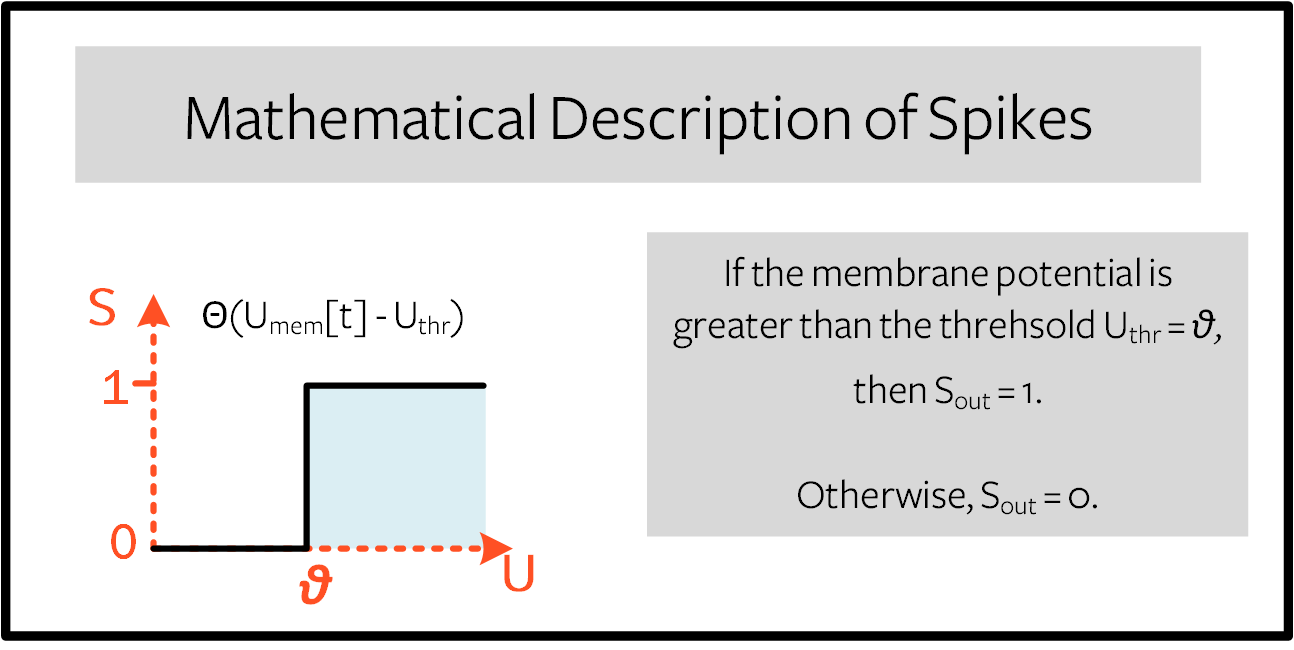
\includegraphics[width=\textwidth]{./image/spike_description.png}
    \caption{Mathematical description of a Spike\cite{eshraghian2021training}}
    \label{fig:spike_description}
  \end{minipage}
\end{figure}

Building upon this foundation, the current report will delve deeper into the intricacies of SNNs, specifically addressing the non-differentiability issue inherent in these networks. Non-differentiability poses a challenge in applying traditional gradient-based optimization techniques commonly used in training Artificial Neural Networks (ANNs). We will explore strategies to tackle this issue and optimize SNNs effectively.

Furthermore, we will introduce the concept of Convolutional Spiking Neural Networks (CSNNs), extending the discussion beyond simple SNN architectures. CSNNs leverage the spatial hierarchies present in convolutional neural networks (CNNs) and integrate them with the temporal dynamics of SNNs. This fusion holds promise for tasks like image recognition, where both spatial and temporal features play crucial roles.

In the practical implementation section, we will present a small program showcasing our results. This program will include the application of CSNNs in a specific task, demonstrating the capabilities and potential advantages of this hybrid architecture.

Throughout this report, our aim is to provide a comprehensive understanding of the advancements and challenges in the realm of Spiking Neural Networks, offering insights into their unique characteristics and applications.

\pagebreak

\section{Reminder on Spikes and Spiking Neural Networks}

Through this section, we aim to provide a comprehensive and visual view of the concepts and mechanisms behind Spiking Neural Networks (SNNs). We will start by revisiting the fundamental aspects of spikes and their encoding, followed by an overview of neuron models (more specifically the Leaky Integrate-and-Fire (LIF) neuron model). We will then delve into the architecture of SNNs and their convolutional variant, Convolutional Spiking Neural Networks (CSNNs).

\subsection{Spikes encoding}

The idea behind spikes is simple: we need to encode some data (let's say an image) into some other kind of data that has a temporal dependency. To do so, we will need to define time steps, a number of steps, and a threshold.
In a rate encoding scheme, we take the values of the pixels of the image and make them pass through a function that will output or not a spike (for example, a Bernoulli function).


\begin{figure}[ht]
  \centering
  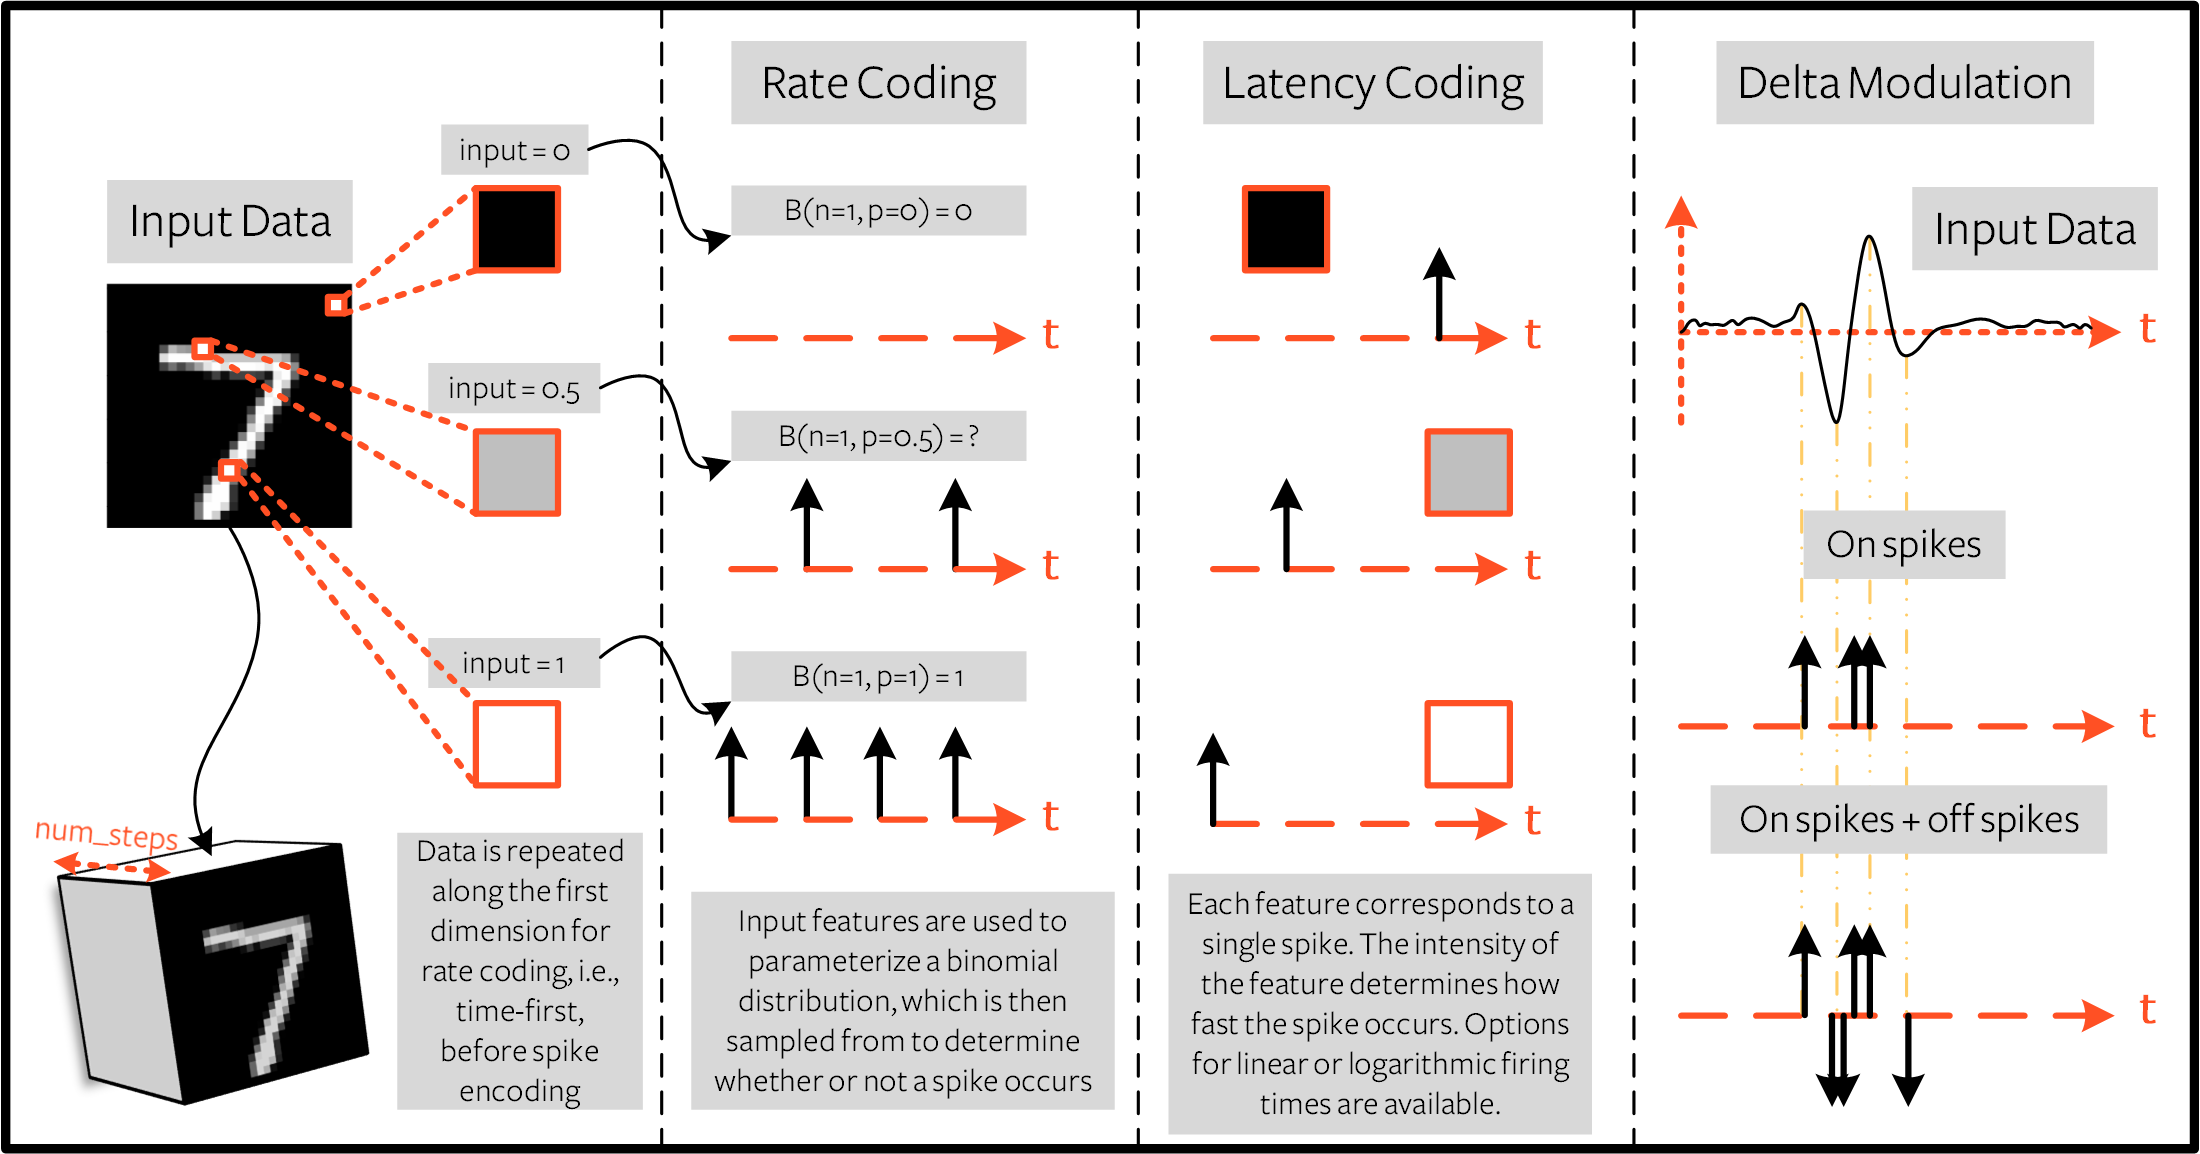
\includegraphics[width=\textwidth]{./image/spikeconv.png}
  \caption{Spike encodings of an image \cite{eshraghian2021training}}
  Source : \url{https://snntorch.readthedocs.io/en/latest/tutorials/tutorial_1.html}
  \label{fig:spikeconversion}
\end{figure}

\subsubsection{Rate encoding}

\subsubsection*{Example}

Let's say we have a white pixel (value close to $1$) and a black pixel (value close to $0$). We will then pass these values through a Bernoulli function with a threshold of $0.5$, if the value is above $0.5$, we will probably output a spike ($1$); if not, we will output $0$.

This way, we end up with an approximation of the image in the form of spikes (binary values !). In order for it to be efficient, we will need encode the image multiple times. So, we will encode the image using the same method but with different time steps:

\begin{figure}[H]
  \centering
  \begin{minipage}{0.3\textwidth}
    \centering
    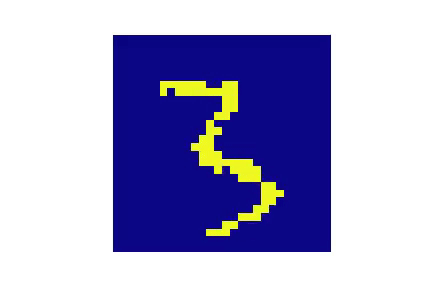
\includegraphics[width=1\textwidth]{image/rate_gif-0.png}
    \caption{MNIST\cite{eshraghian2021training} $t=0$}
    \label{fig:rate_t_0}
  \end{minipage}
  \hfill
  $\xrightarrow{\hspace*{0.3cm}}$
  \hfill
  \begin{minipage}{0.3\textwidth}
    \centering
    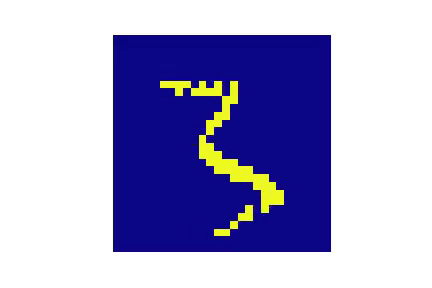
\includegraphics[width=1\textwidth]{image/rate_gif-15.png}
    \caption{MNIST\cite{eshraghian2021training} $t=15$}
    \label{fig:rate_t_15}
  \end{minipage}
  \hfill
  $\xrightarrow{\hspace*{0.3cm}}$
  \hfill
  \begin{minipage}{0.3\textwidth}
    \centering
    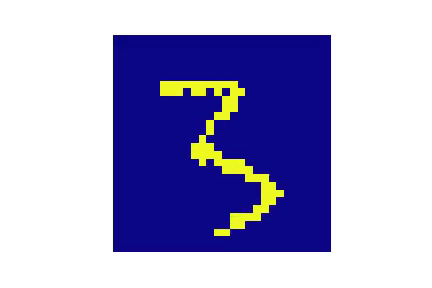
\includegraphics[width=1\textwidth]{image/rate_gif-32.png}
    \caption{MNIST\cite{eshraghian2021training} $t=32$}
    \label{fig:rate_t_32}
  \end{minipage}
\end{figure}

We would define a number of time steps $n_{\text{steps}}$ and encode the image $n_{\text{steps}}$ times. The more time steps we have, the more precise the encoding will be :

\begin{figure}[H]
  \begin{center}
    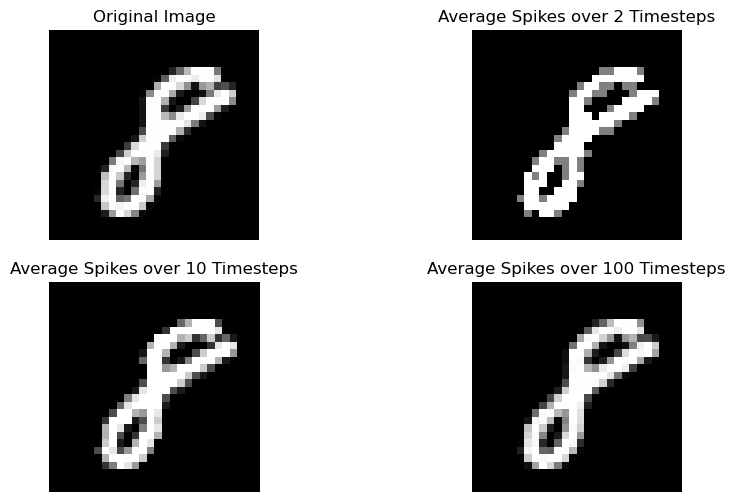
\includegraphics[width=0.8\textwidth]{./image/avg_mnist_spike.png}
    \caption{Average of the encoding of the MNIST dataset}
    \label{fig:avg_mnist_spike}
  \end{center}
\end{figure}

\subsubsection{Latency encoding}

\subsubsection{Delta Modulation}

\subsection{Spiking neuron models}

Until now, we have only talked about the encoding of the data. But another important aspect of Spiking neural network would concern the transmission of spikes and their associated information to the next layer.

We can basically distinguish three phases in a spiking neural network :
\begin{itemize}
  \item Encoding the data into spikes
  \item Transmitting the spikes (and their associated information) to the next layer
  \item Decoding the spikes into a meaningful output
\end{itemize}

To do so, we would need a type of neuron that "fires" spikes when it receives enough input (whatever the inputs are). One might find different kinds of neurons, each with its own characteristics and properties.

\begin{figure}[H]
  \begin{center}
    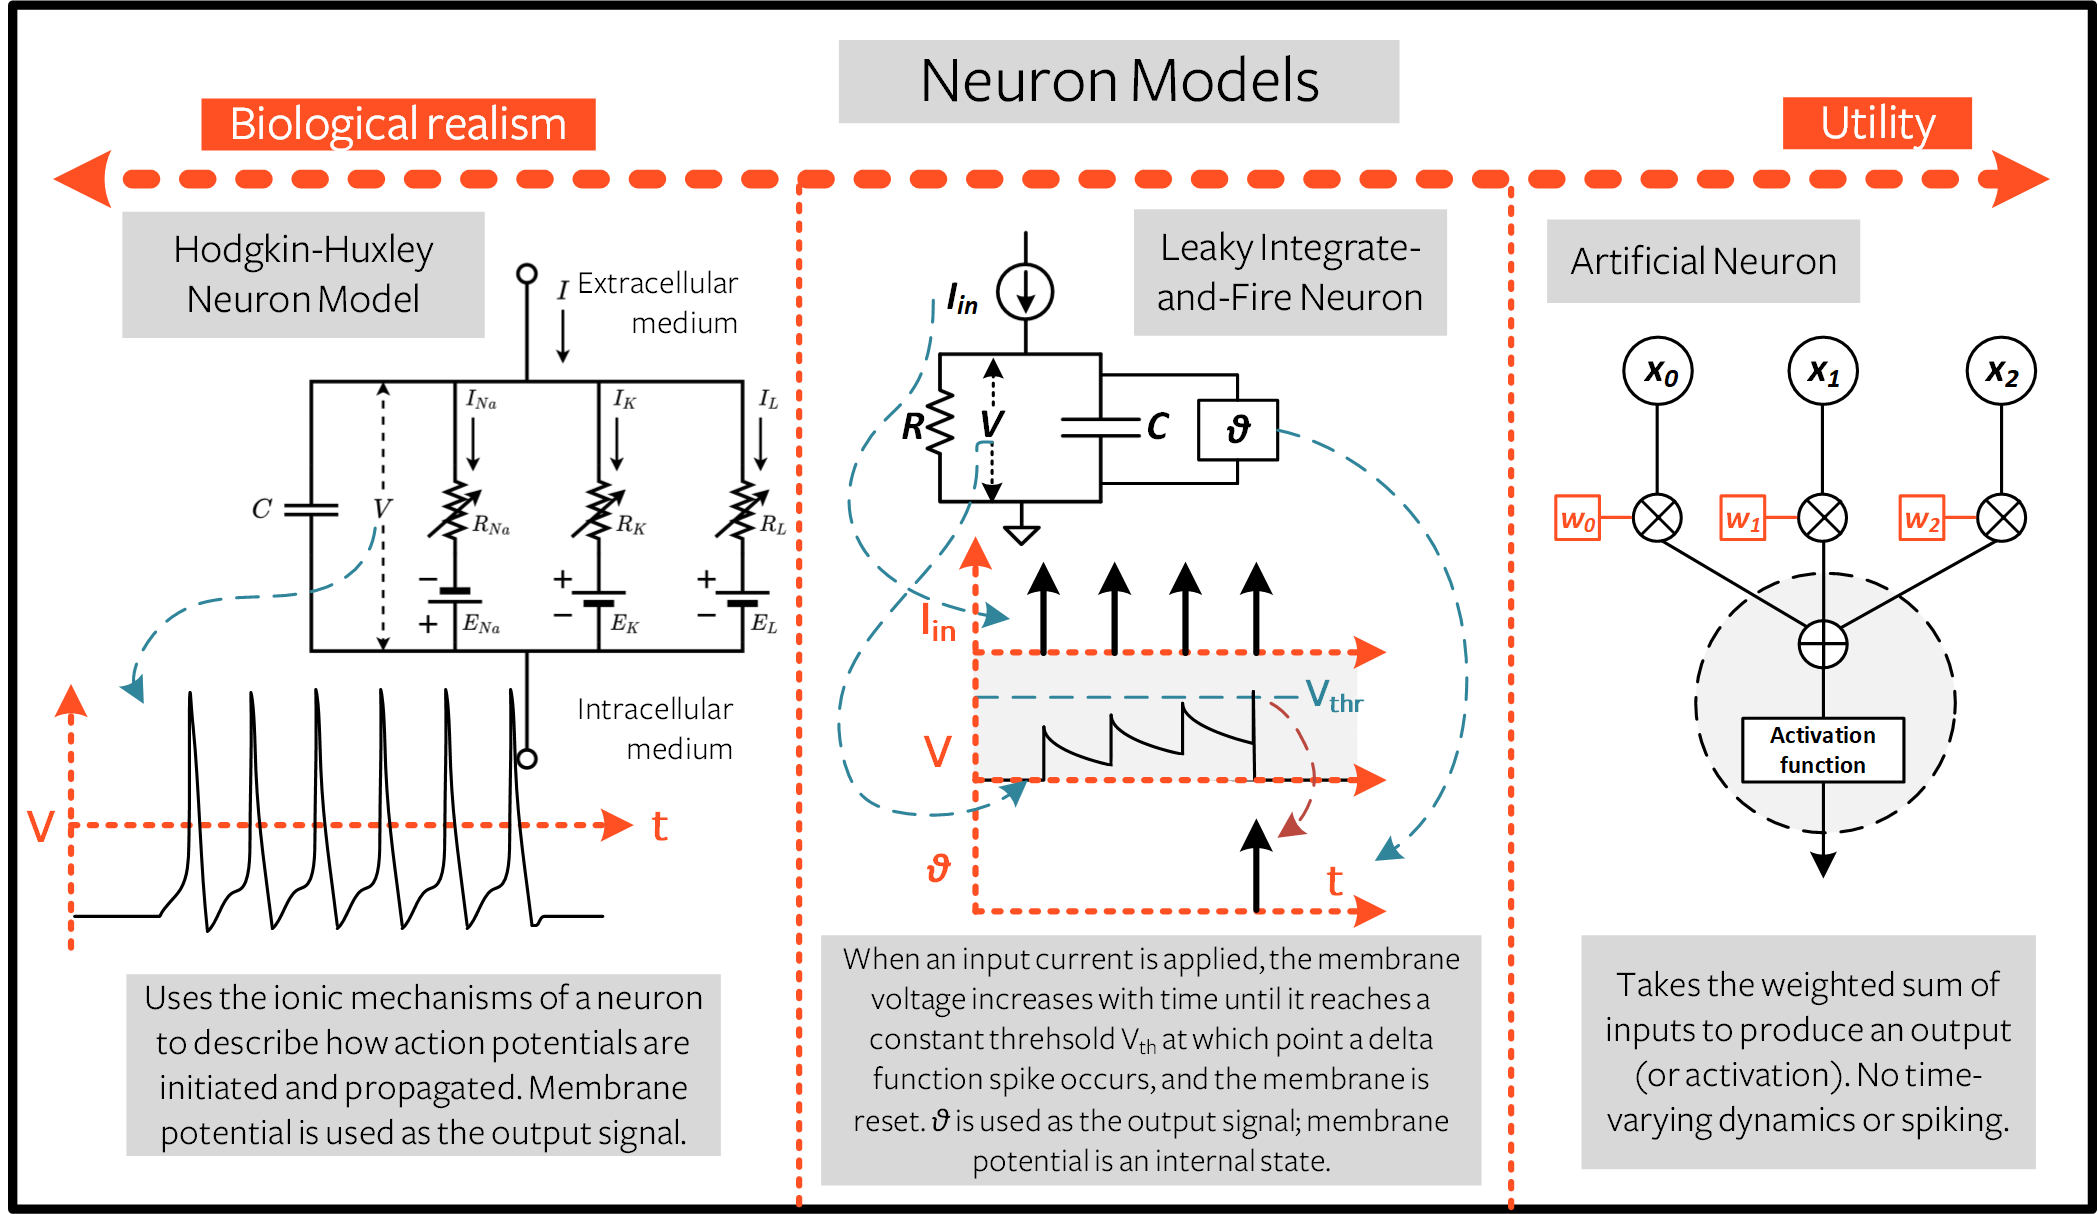
\includegraphics[width=\textwidth]{./image/2_1_neuronmodels.png}
    \caption{Neuron models with schemes}
    \label{fig:neuronmodels_schemes}
  \end{center}
\end{figure}

Bien comme ref : \url{https://neuronaldynamics.epfl.ch/online/}

\subsubsection{Comparison of the different neuron models}

\begin{figure}[H]
  \begin{center}
    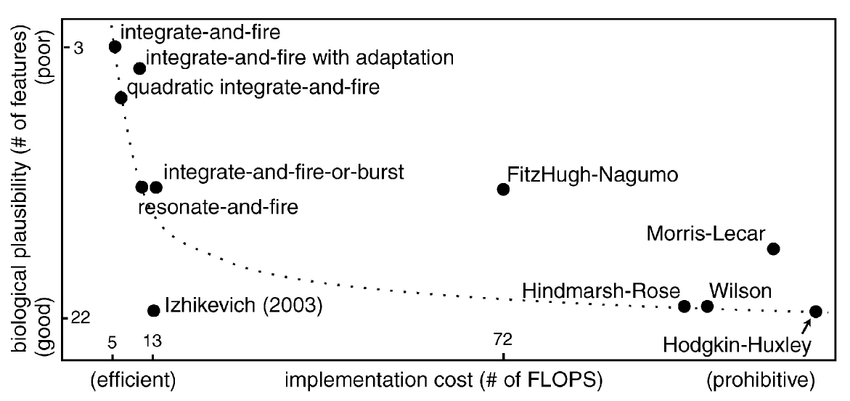
\includegraphics[width=0.8\textwidth]{./image/comparison_neuron.png}
    \caption{Comparison of the different neuron models}
    \label{fig:comparison_neuron}
    Source: \url{https://www.researchgate.net/figure/Trade-off-between-biological-plausibility-with-respect-to-a-number-of-features-known-to_fig3_320409442}
  \end{center}
\end{figure}

\subsubsection{The choice of the Leaky Integrate-and-Fire Neuron Model}

Initially, the LiF model was made as a simple model to mimic the behavior of a neuron.
\begin{quote}
  "In order to arrive at an equation that links the momentary voltage $u_i(t) - u_{rest}$ to the input current $I(t)$, we use elementary laws from the theory of electricity. A neuron is surrounded by a cell membrane, which is a rather good insulator. If a short current pulse $I(t)$ is injected into the neuron, the additional electrical charge $q= \int I(t')dt'$ has to go somewhere: it will charge the cell membrane. The cell membrane therefore acts like a capacitor of capacity $C$. Because the insulator is not perfect, the charge will, over time, slowly leak through the cell membrane. The cell membrane can therefore be characterized by a finite leak resistance $R$.

  The basic electrical circuit representing a leaky integrate-and-fire model consists of a capacitor $C$ in parallel with a resistor $R$ driven by a current $I(t)$ (cf the LiF \hyperref[fig:comparison_neuron]{"Neuron models with schemes"})"\cite{gerstner2014neuronal}
\end{quote}

\begin{figure}[H]
  \begin{minipage}{0.5\textwidth}
    \centering
    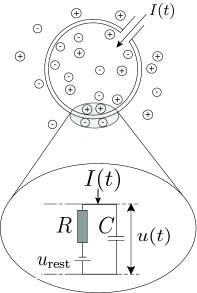
\includegraphics[width=0.6\linewidth]{image/x12.png}
    \caption{A neuron, which is enclosed by the cell membrane (big circle), receives a (positive) input current $I(t)$
      which increases the electrical charge inside the cell. The cell membrane acts like a capacitor in parallel with a resistor which is in line with a battery of potential $u_{rest}$\cite{gerstner2014neuronal}}
    \label{fig:neuron_real_circuit}
  \end{minipage}
  \hspace{0.5cm}
  \begin{minipage}{0.5\textwidth}
    \centering
    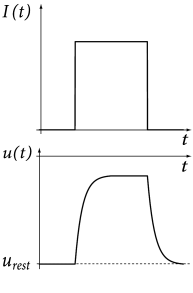
\includegraphics[width=0.6\linewidth]{image/x13.png}
    \caption{The cell membrane reacts to a step current (top) with a smooth voltage trace (bottom)\cite{gerstner2014neuronal}}
    \label{fig:neuron_real_circuit_trace}
  \end{minipage}
\end{figure}

\subsubsection{Leaky Integrate-and-Fire Neuron Model}

With the Leaky Integrate-and-Fire (LIF) model been the most used in practice. It can be seen as follows :

\begin{itemize}
  \item We define a membrane potential $U_m$ that will be updated at each time step
        \begin{equation}
          U_m[t+1] = \underbrace{\beta U_m[t]}_\text{decay} + \underbrace{WX[t+1]}_\text{input} - \underbrace{S[t]U_{\rm thr}}_\text{reset}  \quad \text{\cite{eshraghian2021training}}
        \end{equation}

  \item We define a threshold $U_{\rm thr}$ that will be used to reset the membrane potential when it is reached
  \item The output spike will be emitted following the following equation :
        \begin{equation}
          S(t) = \begin{cases}
            1 & \text{if } U_m(t) \geq U_{\rm thr} \\
            0 & \text{otherwise}
          \end{cases}
        \end{equation}
\end{itemize}

\begin{figure}[H]
  \begin{minipage}{0.5\textwidth}
    \begin{figure}[H]
      \begin{center}
        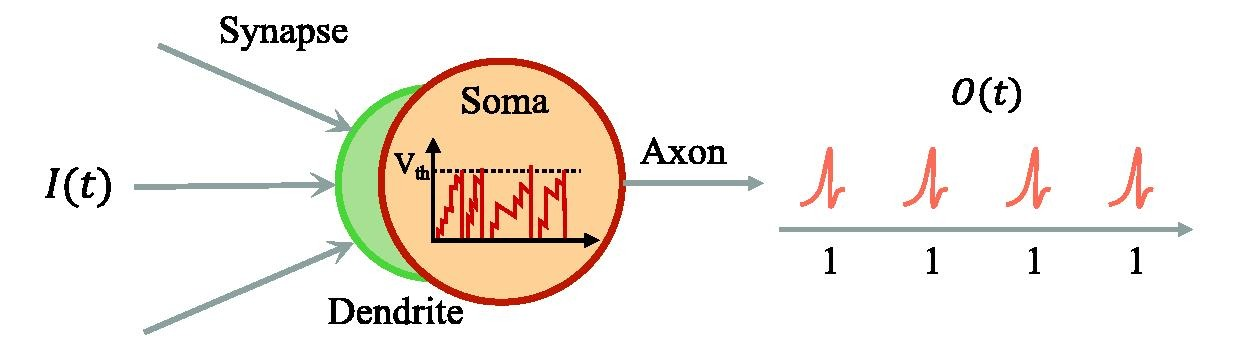
\includegraphics{image/neuronmodel.jpg}
        \caption{Neuron model basis\cite{LIAO2023126470}}
        \label{fig:neuronmodel}
      \end{center}
    \end{figure}
  \end{minipage}
  \hspace{0.5cm}
  \begin{minipage}{0.5\textwidth}
    \begin{center}
      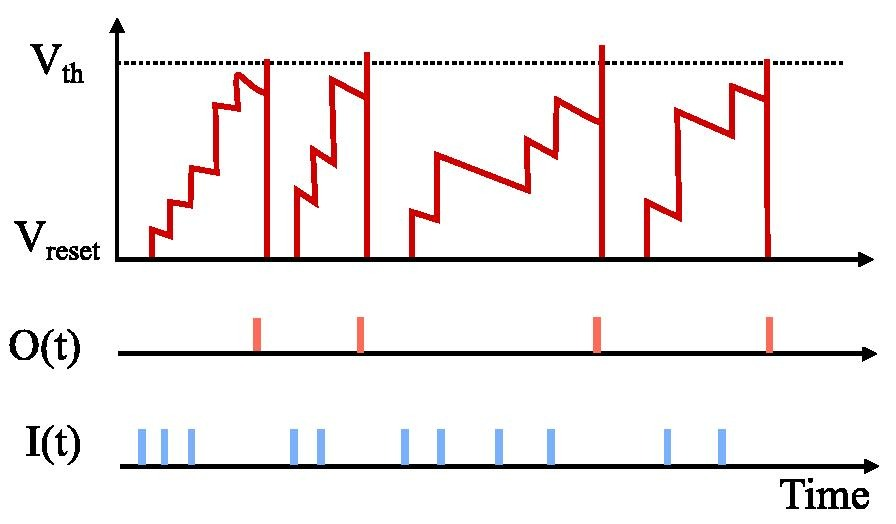
\includegraphics{image/generating_spikes.jpg}
      \caption{Generating spikes\cite{LIAO2023126470}}
      \label{fig:generating_spikes}
    \end{center}
  \end{minipage}
\end{figure}

% algo LIF
The algorithm defining the Lif neuron model in Snntorch have the following structure :
\begin{algorithm}
  \caption{Snntorch : Leaky Integrate-and-Fire Neuron Model}
  \begin{algorithmic}[1]
    \Require $input$, $mem_0$
    \State Initialize $beta$, $threshold$, $spike\_grad$, $surrogate\_disable$, $init\_hidden$, $inhibition$, $learn\_beta$, $learn\_threshold$, $reset\_mechanism$, $state\_quant$, $output$
    \State Initialize $Leaky.beta$ and $Leaky.threshold$ if they are learnable
    \For{each $input$ in $batch$}
    \If{$reset\_mechanism = "subtract"$}
    \EndIf
    \State Compute $U[t+1] = \beta U[t] + I_{in}[t+1] - RU_{thr}$ if $reset\_mechanism = "subtract"$
    \State Compute $U[t+1] = \beta U[t] + I_{syn}[t+1] - R(\beta U[t] + I_{in}[t+1])$ if $reset\_mechanism = "zero"$
    \State Compute $spk$ and $mem_1$ for each element in the batch
    \State Return $spk$ and $mem_1$
    \EndFor
  \end{algorithmic}
\end{algorithm}

In pratcice, when using Snntorch we would create 2 arrays, one for the membrane potential and one for the spikes.

TODO

\subsection{Spiking Neural Networks}

\subsection{Convolutional Spiking Neural Networks}

\pagebreak

\section{SNN - Behind the scenes}

\subsection{How to train a SNN}

\subsection{Dead Neuron Problem}

\begin{wrapfigure}{r}{0.6\textwidth}
  \centering
  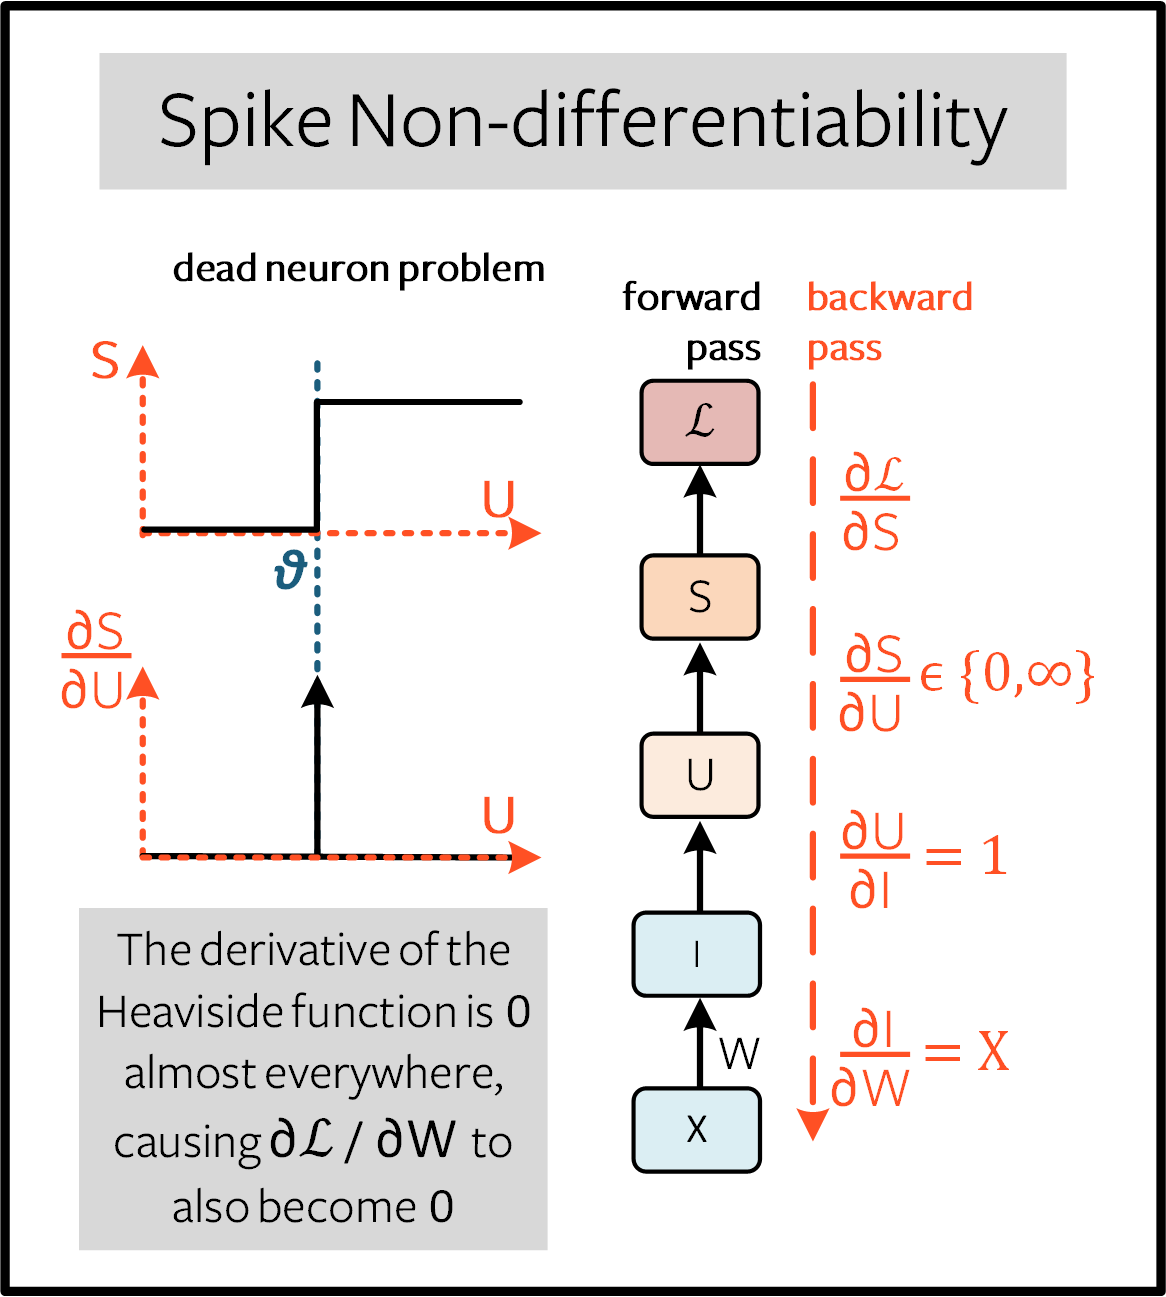
\includegraphics[width=0.6\textwidth]{./image/non-differentiability.png}
  \caption{Dead neuron problem\cite{eshraghian2021training}}
\end{wrapfigure}

To train a spiking neural network, we aim to adjust the weights based on the loss gradient, minimizing the overall loss. Backpropagation achieves this through a chain of derivatives:

$$
  \frac{\partial \mathcal{L}}{\partial W} =
  \frac{\partial \mathcal{L}}{\partial S}
  \underbrace{\frac{\partial S}{\partial U}}_{\{0, \infty\}}
  \frac{\partial U}{\partial I}
  \frac{\partial I}{\partial W}
$$

Here, $\mathcal{L}$ is the loss, $W$ represents weights, $S$ is the output, $U$ is the activation function, and $I$ is the input.

The challenge lies in the term $\frac{\partial S}{\partial U}$, which takes values between $0$ and $\infty$. The derivative of the Heaviside step function from the input ($U$) is the Dirac Delta function. This function is $0$ everywhere except at the threshold $\theta$, where it tends to infinity. Consequently, the gradient is often nullified to zero (or saturated if $\theta$ precisely aligns with the threshold), hindering learning. This issue is commonly known as the \textbf{dead neuron problem}. There are multiple ways to address this issue.

\subsection{Shadow training}

\subsection{Surrogate Gradient}

One way to address this non-differentiability issue would be to compute a gradient on a "relaxed" version of the non-differentiable function. This would mean approximating the Heaviside step function $S(U)$ with a differentiable function $f(U)$, such as the sigmoid function or the $\arctan$ function. For example:

\begin{figure}[ht]
  \begin{minipage}[t]{0.5\textwidth}
    \vspace{40pt} % Adjust this value as needed
    $$\begin{aligned}
        S(U) & \approx \frac{1}{1 + e^{-\beta(U - \theta)}}       \\
             & \text{Or alternatively}                            \\
        S(U) & \approx \frac{1}{\beta} \arctan(\beta(U - \theta))
      \end{aligned}$$
  \end{minipage}
  \hfill
  \begin{minipage}[t]{0.45\textwidth}
    \vspace{0pt} % Adjust this value as needed
    \centering
    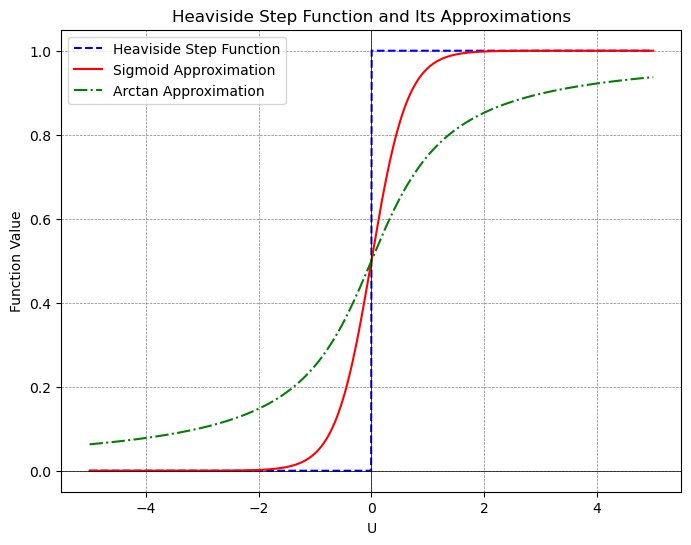
\includegraphics[width=\textwidth]{./image/approx_surrogate.png}
    \caption{Visualization of the Heaviside step function approximation\cite{LIAO2023126470}}
    \label{fig:approx_surrogate}
  \end{minipage}
\end{figure}

\subsubsection{Loss function treatment}

In order for this to be taken into account in the loss function (and because we now have to take the time as a parameter), we have to perform an operation on the loss function for all its time steps.

$$ \frac{\partial \mathcal{L}}{\partial W}=\sum_t \frac{\partial\mathcal{L}[t]}{\partial W} =
  \sum_t \sum_{s\leq t} \frac{\partial\mathcal{L}[t]}{\partial W[s]}\frac{\partial W[s]}{\partial W}$$

\section{Practical implementation}

\pagebreak

% Bibliography
\bibliographystyle{siam}
\bibliography{ref}


\end{document}
